\documentclass[11pt,handout]{beamer}
\usetheme{Warsaw}
\usepackage[utf8]{inputenc}
\usepackage[french]{babel}
\usepackage[T1]{fontenc}
\usepackage{amsmath}
\usepackage{amsfonts}
\usepackage{amssymb}
\usepackage{graphicx}
\hypersetup{pdfpagemode=FullScreen}
\author[Ramadan SOUMAILA]{}
\title{Système de géolocalisation sur le campus d'Abomey-Calavi}
\setbeamercovered{transparent} 
%\setbeamertemplate{navigation symbols}{} 
\logo{} 
\institute{} 
\date{} 
%\subject{}
\begin{document}
\begin{frame}
	\begin{center}
	
\includegraphics[scale=0.15]{images/logoUAC1.png}
	 \hspace{1.1cm}
	  {\scriptsize \textbf{\textsf{UNIVERSITÉ D'ABOMEY-CALAVI}}}
	   \hspace{1.1cm}
	   
\includegraphics[scale=0.15]{images/logoIfri.png}\\
	  {\footnotesize \textbf {\textsf{INSTITUT DE FORMATION ET DE RECHERCHE EN INFORMATIQUE}}}
	\end{center}
	\begin{center}
		\titlepage
		Présenté par : Ramadan \textbf{SOUMAILA\\}
		Sous la supervision de : Prof Eugène C. \textbf{EZIN}
	\end{center}
\end{frame}
	\section{Contexte et Problématique}
		\subsection{Problématique}
			\begin{frame}
			    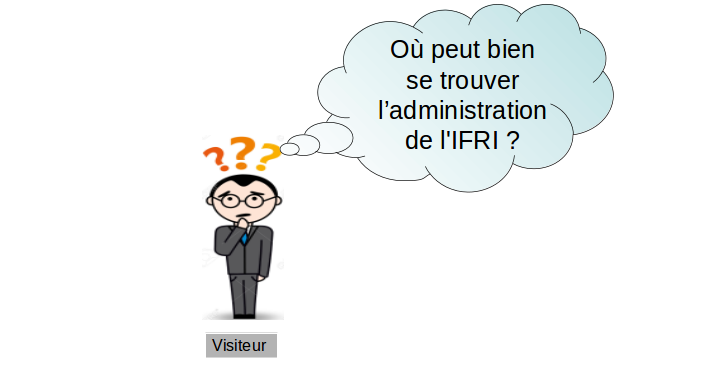
\includegraphics[scale=0.5]{images/problematique_1.png}
			\end{frame}
			\begin{frame}
			    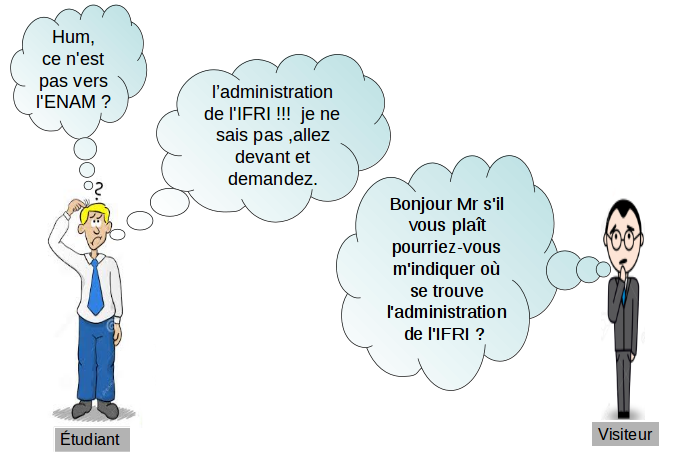
\includegraphics[scale=0.45]{images/preuve_2.png}
			\end{frame}
	\section{Présentation de UAC Géolocalisation}
		      \begin{frame}
			  \hspace{0.7cm}
			  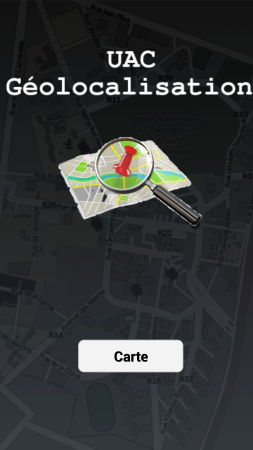
\includegraphics[scale=0.45]{images/accueil.png}
			  \hspace{0.5cm}
			  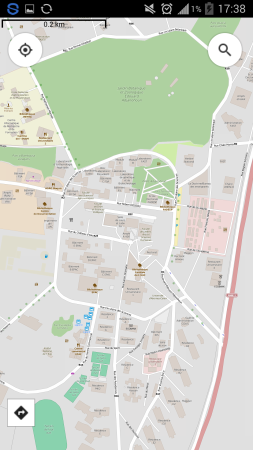
\includegraphics[scale=0.45]{images/carte.png}
		      \end{frame}
		      
		       \begin{frame}

			  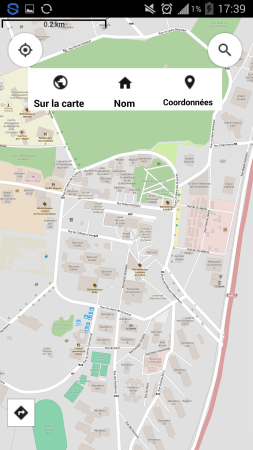
\includegraphics[scale=0.42]{images/recherche.png}
			  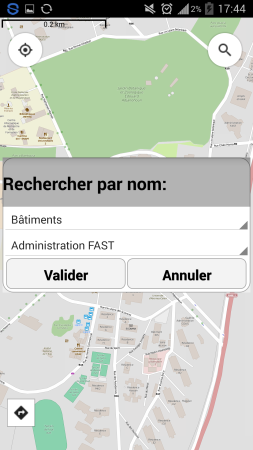
\includegraphics[scale=0.42]{images/par_nom.png}
			   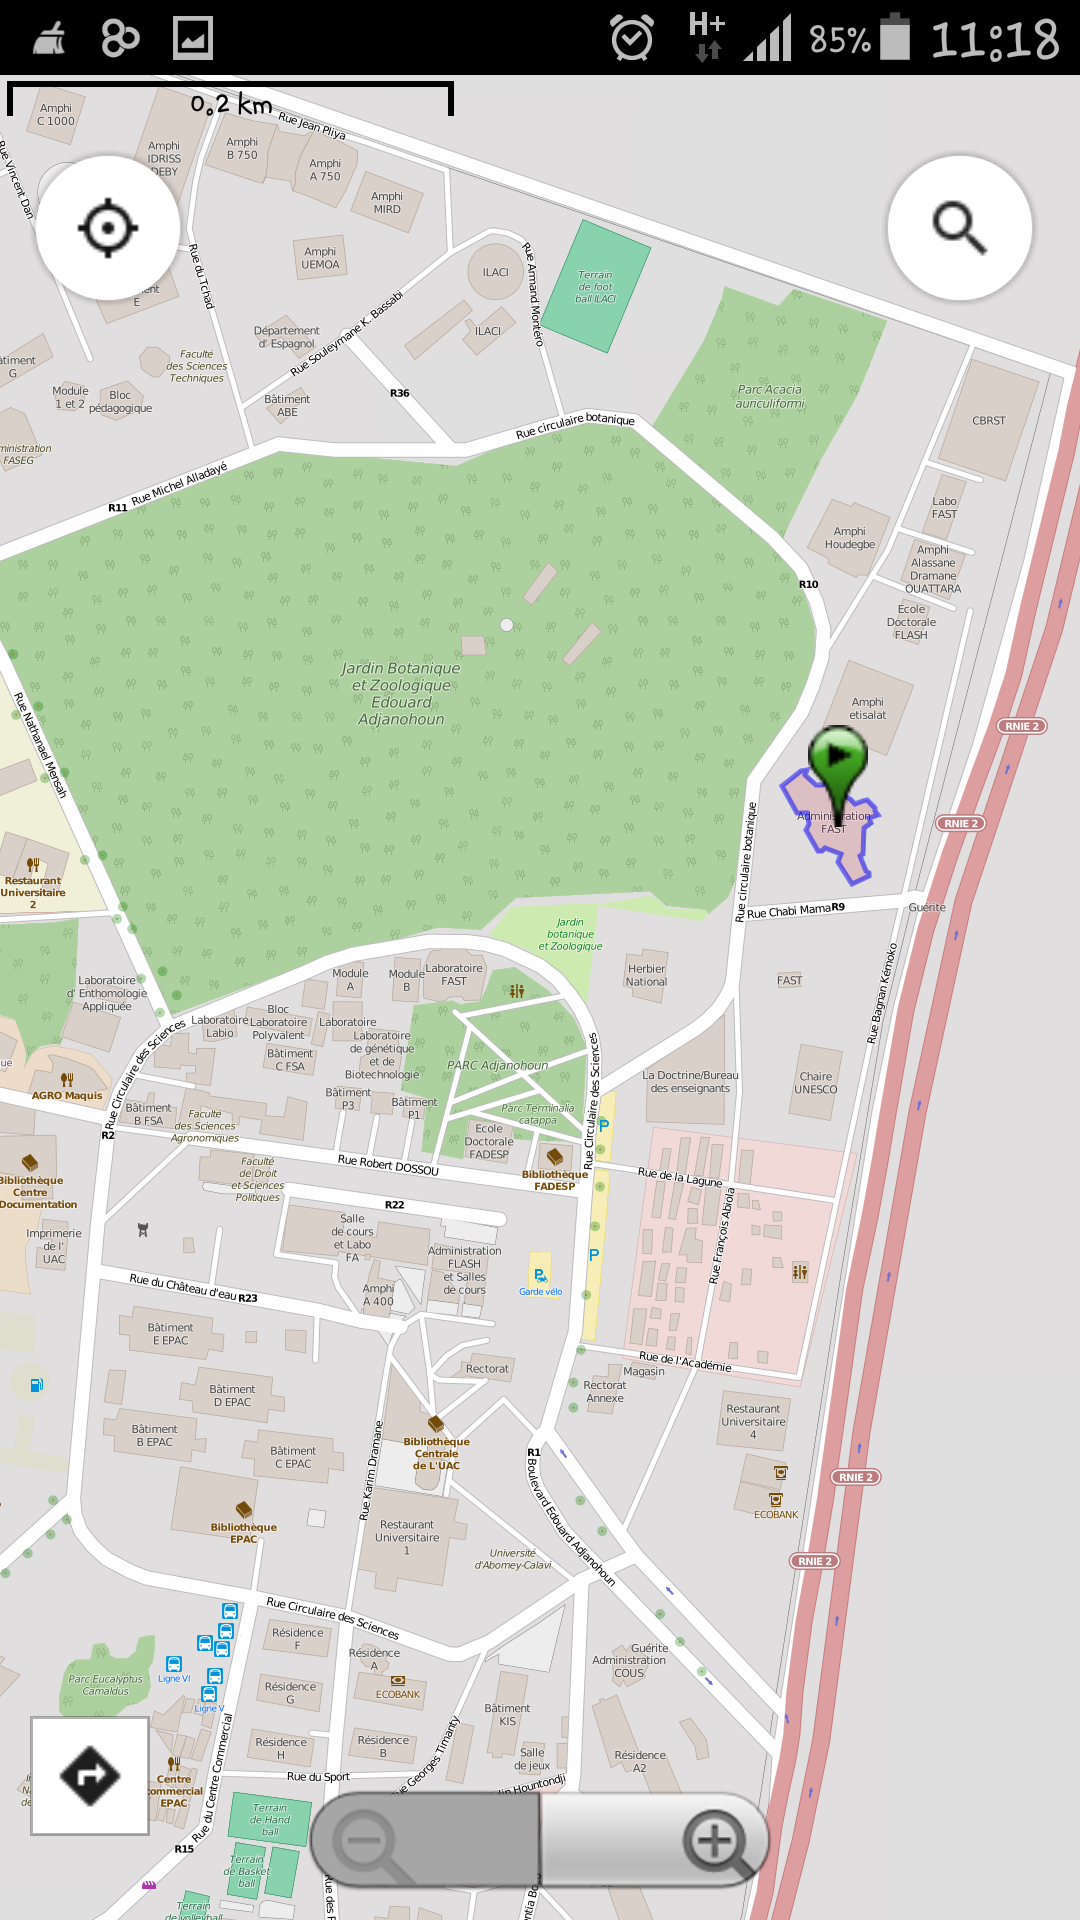
\includegraphics[scale=0.0985]{images/cherche_result.png}
		      \end{frame}
		      
		       \begin{frame}
			  \hspace{1.5cm}
			  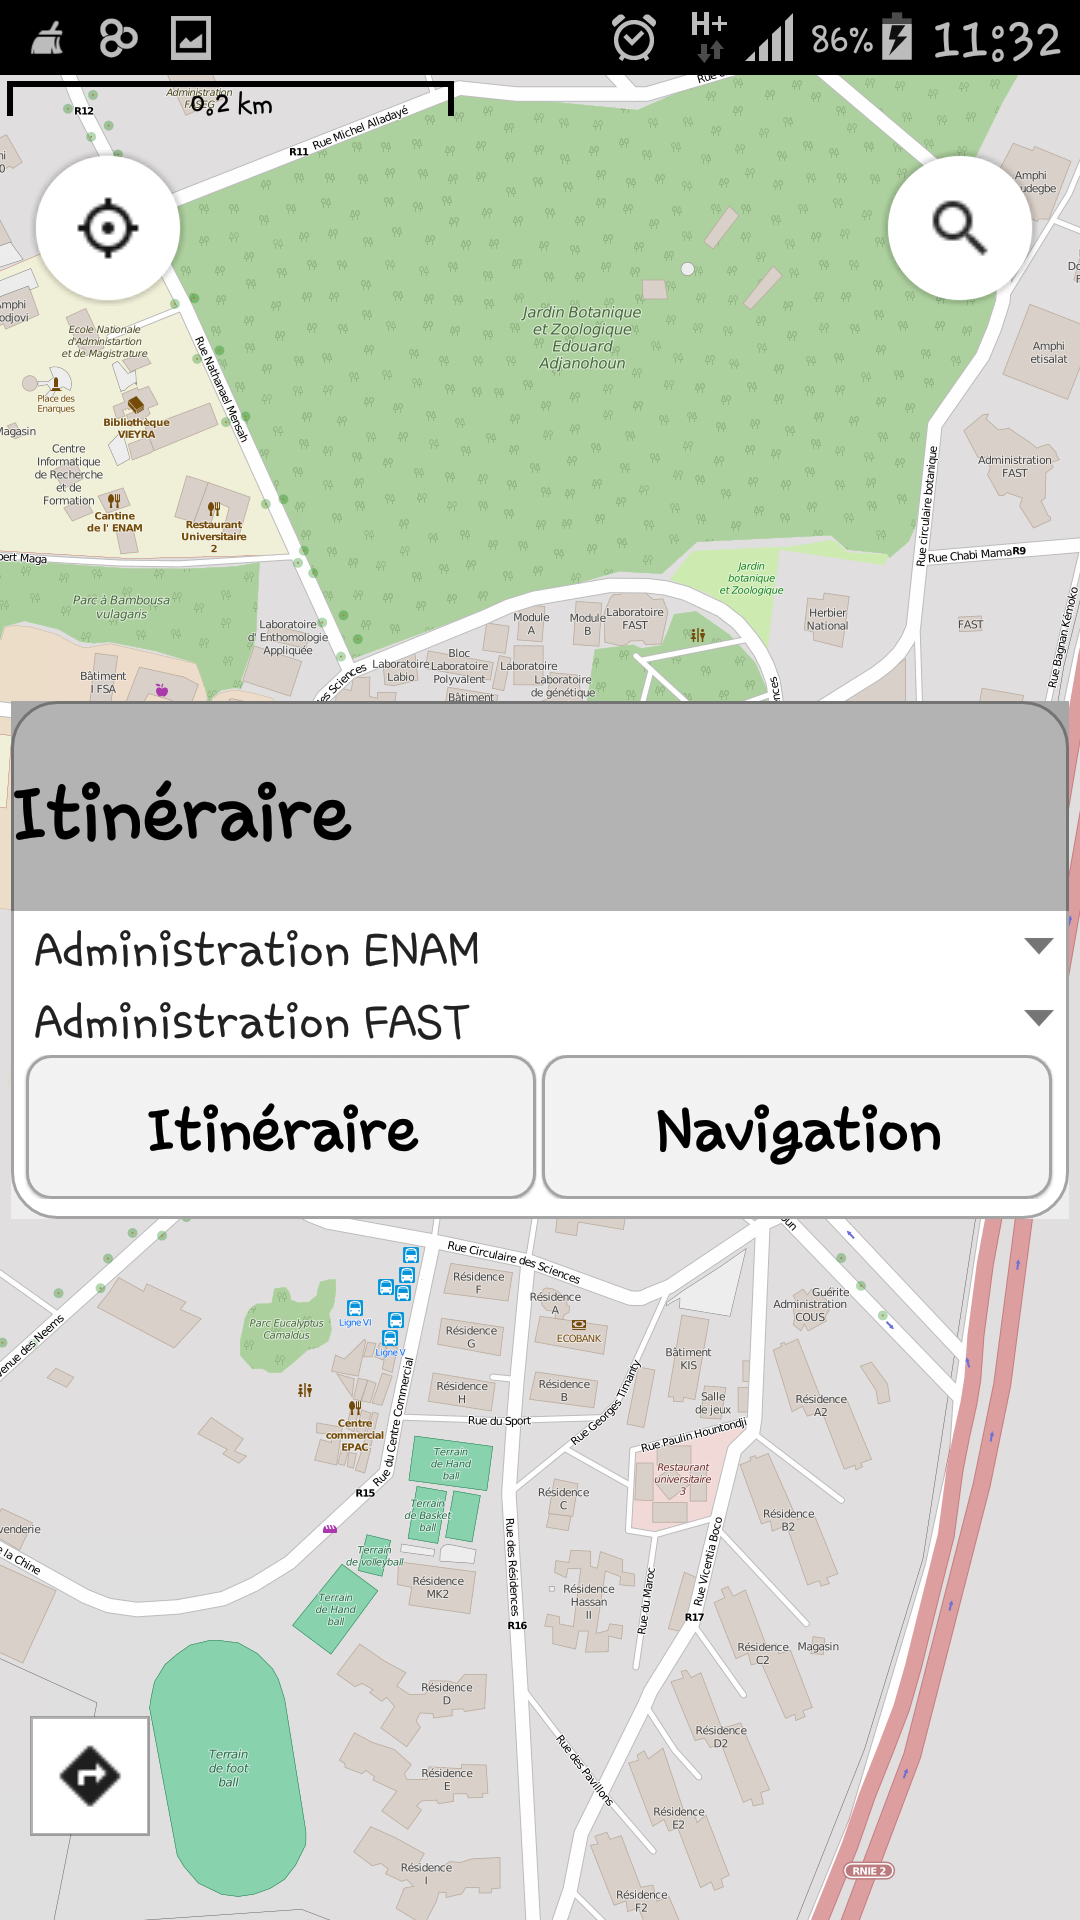
\includegraphics[scale=0.1]{images/Itin_cher.png}
			  \hspace{0.5cm}
			  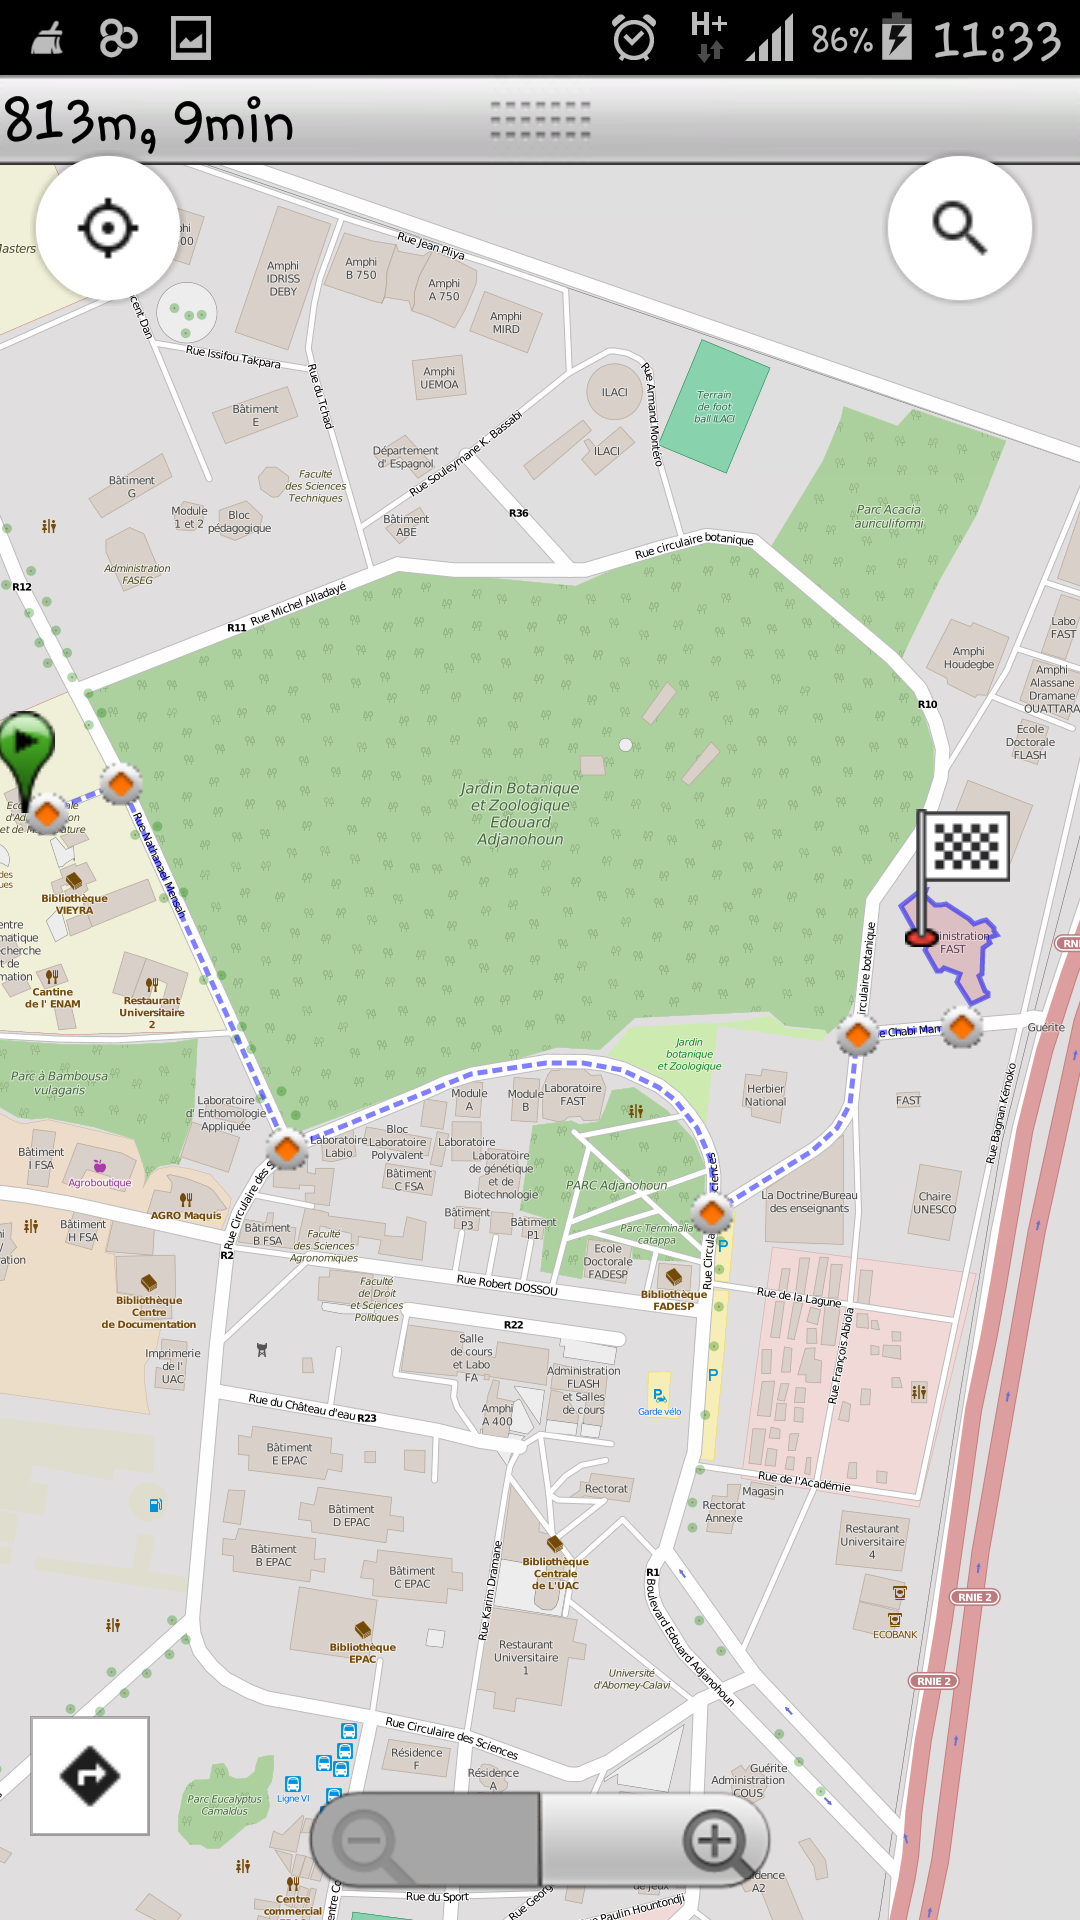
\includegraphics[scale=0.1]{images/Itin_result.png}
		      \end{frame}

\end{document}}